\documentclass[10pt, hyperref={unicode}, utf8x]{beamer}
\usepackage[czech]{babel}
\usepackage{hyperref}
\usepackage[ruled, czech, noline, linesnumbered, noend]{algorithm2e}
\usepackage{graphics}

\usetheme{Madrid}
\makeatletter
\setbeamertemplate{footline}
{
  \leavevmode%
  \hbox{%
  \begin{beamercolorbox}[wd=.333333\paperwidth,ht=2.25ex,dp=1ex,center]{author in head/foot}%
    \usebeamerfont{author in head/foot}\insertshortauthor
  \end{beamercolorbox}%
  \begin{beamercolorbox}[wd=.333333\paperwidth,ht=2.25ex,dp=1ex,center]{title in head/foot}%
    \usebeamerfont{title in head/foot}\insertshorttitle
  \end{beamercolorbox}%
  \begin{beamercolorbox}[wd=.333333\paperwidth,ht=2.25ex,dp=1ex,right]{date in head/foot}%
    \usebeamerfont{date in head/foot}\insertshortdate{}\hspace*{2em}
    \insertframenumber{} / \inserttotalframenumber\hspace*{2ex} 
  \end{beamercolorbox}}%
  \vskip0pt%
}
\makeatother

\title{Grafové algoritmy}
\subtitle{Typografie a publikování 5. projekt}
\author{Denis Kramár}
\date{\today}
\institute{
    Vysoké učení technické v Brně\\
    Fakulta informačních technologií
}


\begin{document}

\maketitle

\frame {
    \frametitle{Obsah}
    \begin{itemize}
        \item Algoritmus Dijkstra
        \item Pseudokód
        \item Dijkstra obrázok
        \item Zdroje
    \end{itemize}
}

\frame {
    \frametitle{Algoritmus Dijkstra}
    \begin{itemize}
        \item Slúži na určenie najkratšej vzdialenosti medzi počiatočným vrcholom a iným vrcholom v grafe
        \item Podstata algoritmu je v kontunuálnom výpočte najkratšej vzdialenosti a vylúčenie dlhších vzdialeností pri aktualizácii
    \end{itemize}
}

\frame{
    \frametitle{Pseudokód}
    \IncMargin{3em}
	\begin{algorithm}[H]
		\caption{\textsc{Dijkstra}}
		\SetKwRepeat{Do}{do}{while}%
		\SetKwFunction{FMain}{Dijkstra}
		\SetKwProg{Pn}{function}{:}{\KwRet}
        \Pn{\FMain{Graph, source}}{
            \ForEach{vertex v in Graph}{
                dist[v] := infinity \\
                previous[v] := undefined \\
            }
            
            dist[source] := 0 \\
            Q := the set of all nodes in Graph \\
            \While{Q \textbf{is not} empty}{
                u := node in Q with smallest dist[] \\
                remove u from Q \\
                
                \ForEach{neighbor v of u}{
                    alt := dist[u] + dist\_between(u, v)\\
                    \uIf{alt < dist[v]}{
                        dist[v] := alt \\
                        previous[v] := u \\
                    }
                }
            }
            \Return previous[]
        }
	\end{algorithm}
}

\frame{
    \frametitle{Dijkstra obrázok}
    \centering
    \scalebox{0.4}{
        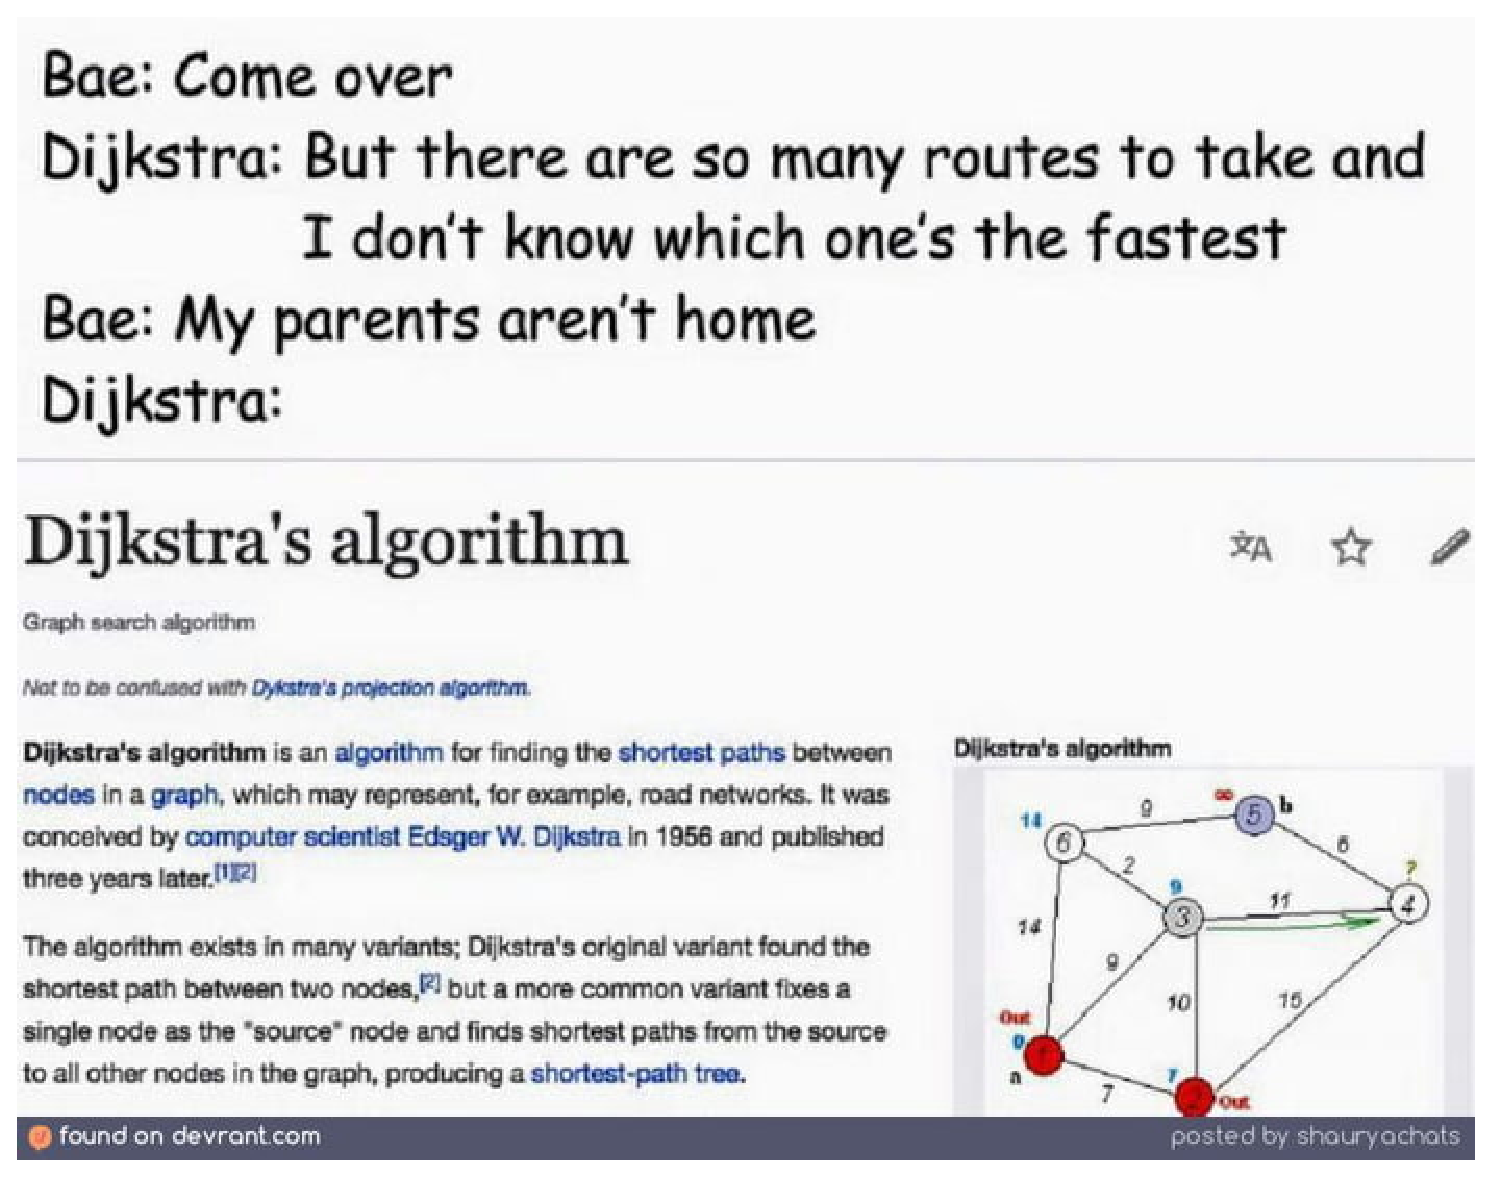
\includegraphics{dijkstra.eps}
    }
}

\frame{
    \frametitle{Použité zdroje}
	\begin{thebibliography}{}
        \bibitem{} GITTA:
            \url{http://www.gitta.info/Accessibiliti/en/html/Dijkstra_learningObject1.html}
        \bibitem{} Math MIT:
            \url{https://math.mit.edu/~rothvoss/18.304.3PM/Presentations/1-Melissa.pdf}  
        \bibitem{} 9GAG:
            \url{https://9gag.com/gag/a8o10zO}
    \end{thebibliography}
}

\frame{
    \centering
    Ďakujem za pozornosť!
}

\end{document}
